%!tex root = ../report.tex

\section{Testing Patterns}

\subsection{Testing}
\textbf{Test Model}\\
Consolidates the following components into one package:
\begin{itemize}
  \item Test Cases/Tests: Description of the testing activities, derived from use cases
  \item Test Driver: Programs executing tests
  \item Input Data
  \item Oracle: Compares expected output with actual output
  \item Test Harness/Testing Framework: Software components/framework
\end{itemize}
\vspace{1em}
\textbf{Model-Based Testing}
Technique, where the system model is used for the generation of the test model.
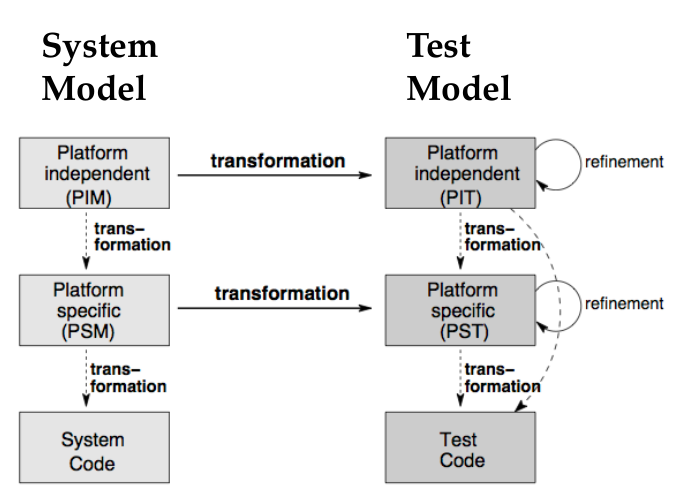
\includegraphics[width=.5\linewidth]{images/testing_generating_test_code}\\
\\
\textbf{Testing Activities}\\
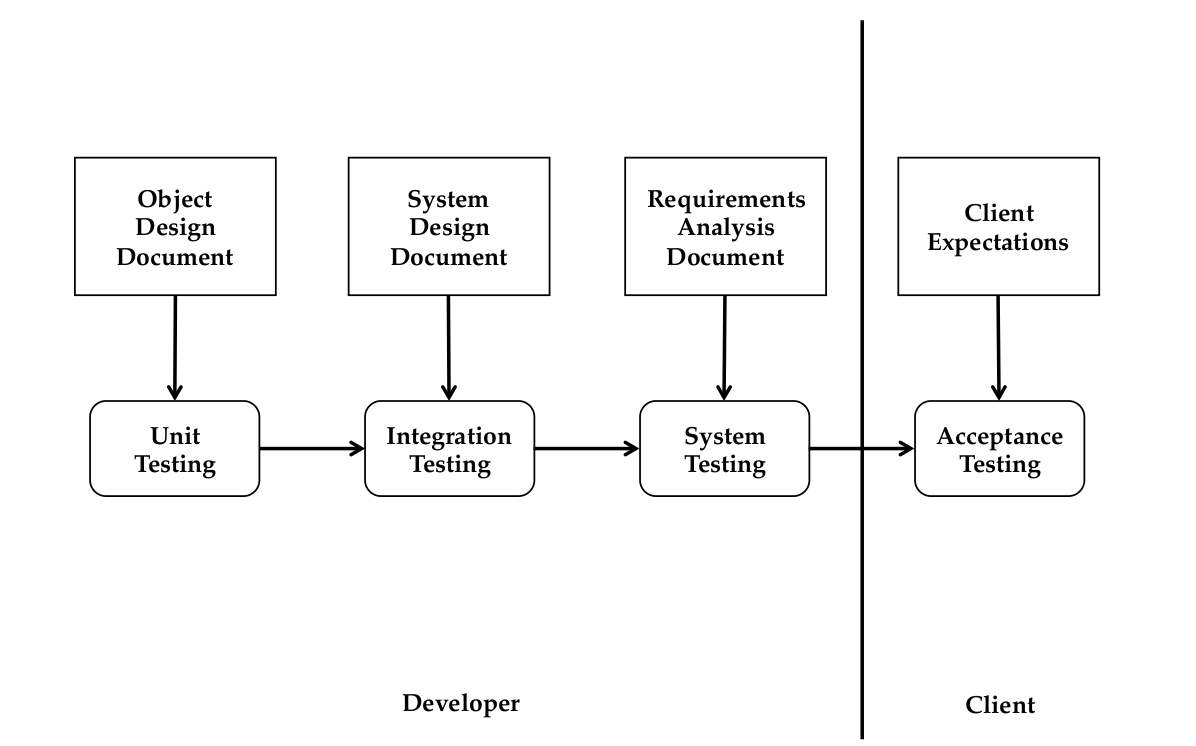
\includegraphics[width=.5\linewidth]{images/testing_activities.png}\\
Regression Testing: Testing after each change
\newpage
\textbf{JUnit Testing}\\
Annotations:
\vspace{-.5em}
\begin{itemize}
  \item @Test public void foo(): foo is a test
  \item @Before public void bar(): bar is executed before every test
  \item @After public void foobar(): Any test method must finish with call to foobar
  \item @BeforeClass public void foofoo(): foofoo is executed before the start of all tests
  \item @AfterClass public void blabla(): blabla is executed after all tests have finished
  \item @Ignore(String s): Ignores the prefixed method and prints s instead
  \item @Test(expected=IllegalArgumentException)
  \item @Test(timeout=100)
\end{itemize}
Assertions:
\vspace{-.5em}
\begin{itemize}
  \item assertTrue(predicate)
  \item assertFalse(predicate)
  \item fail(String): lets the method fail
  \item assertsEquals([String message], expected, actual)
  \item assertsEquals([String message], expected, actual, tolerance): Used for float and double
  \item assertNull([message], object): prints message if object is null
  \item assertNotNull([message], object)
  \item assertSame([String], expected, actual): expected == actual (not equals!)
  \item assertNotSame([String], expected, actual)
\end{itemize}
\newpage

\subsection{Object-Oriented Model-Based Testing}
The test model now contains \textbf{objects} called doubles (from stunt double) that replace classes in the system that have not yet been implemented.\\
There are four types of doubles:
\vspace{-.5em}
\begin{itemize}
  \item \textbf{Dummy Object:} Used to fill parameter holes, never actually used
  \item \textbf{Fake Object:} Functional class, that has not yet the actual functionality of the real class (e.g. database implementation that is stored on the memory only)
  \item \textbf{Stub:} Returns always the same values (e.g. always 42 in a RNG)
  \item \textbf{Mock Object:} Imitates real behavior of an object. Requires a good architecture to let the mock class inherit from the desired interface.
\end{itemize}
\newpage

\subsubsection{Mock-Object Pattern}
Structure:\\
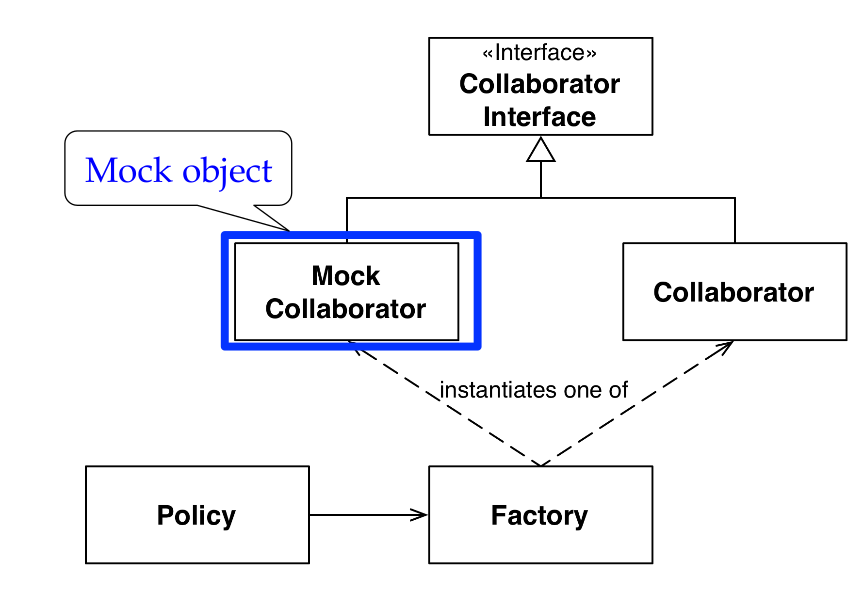
\includegraphics[width=.75\linewidth]{images/testing_pattern_mock_object.png}\\
Applicability:
\begin{itemize}
  \item Unit tests with nondeterministic behavior (e.g. weather)
  \item Object is difficult to set up (e.g. large mazes in a game)
  \item Specific behavior is hard to trigger (e.g. network errors)
  \item Slow methods (e.g. climate modeling)
  \item Object has an user interface or is the user
  \item The real object is not testable
\end{itemize}
Easy Mock:
\begin{enumerate}
  \item Instantiate mock object: mock = createMock(foo.class)
  \item Specify the expected behavior
  \begin{enumerate}
    \item Void methods are called as in Java
    \item For methods with return values: use expect() to specify the return type and andReturn() to specify its value
    \item times() defines how often the method can be called
  \end{enumerate}
  \item Use replay(mock) to make the mock object available
  \item Invoke methods in the SUT (system under test)
  \item Make sure the SUT used the mock object as specified with verify(mock)
\end{enumerate}
\newpage

\subsubsection{Dependency Injection Pattern}
Dependency injection is designed to avoid high coupling between test classes and the SUT.\\
Structure:\\
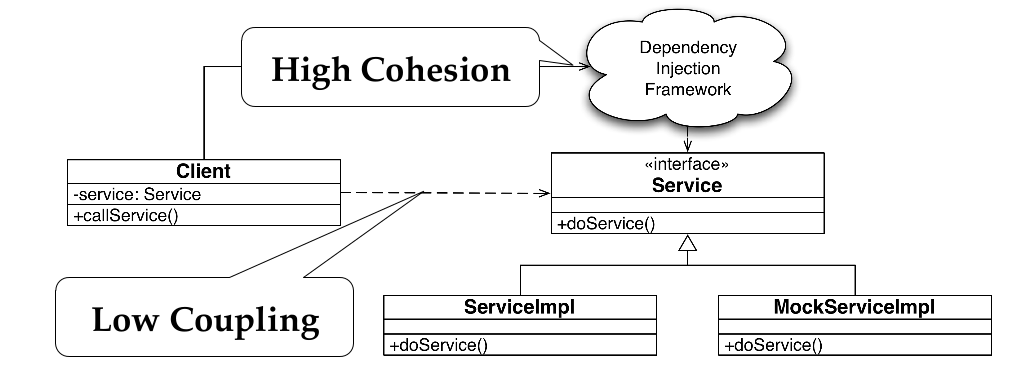
\includegraphics[width=\linewidth]{images/testing_pattern_dependency_injection.png}\\
\textbf{Google Guice Framework:}
\begin{enumerate}
  \item Place the @Inject annotation (constructors, methods, fields)
  \item Create a \textit{Module} to define binding (implement configure()\{bind(Service.class).to(ServiceImpl.class)\})
  \item Instantiate an injector to tell which module to use (Guice.createInjector(new ProductionModule()))
  \item Instantiate an instance of the classed needing injection (injector.getInstance(Service.class))
\end{enumerate}
\newpage
